\documentclass{article}
\usepackage[T1]{fontenc}
\usepackage[utf8]{inputenc}
\usepackage{hyperref}
\usepackage{geometry}
\usepackage{polski}
\usepackage{amsmath}
\usepackage{algorithm2e}
\usepackage{graphicx}

\title{Opis filtru opartego na spreadzie}
\author{Zygmunt Zawadzki}



\begin{document}
\maketitle


%% Spread
\newcommand{\Spt}{\ensuremath{Sp_{t}} }

\newcommand{\MSpc}{\ensuremath{Sp_{t|t-1}} }
\newcommand{\MSpn}{\ensuremath{Sp_{t+1|t}} }
\newcommand{\MSpo}{\ensuremath{Sp_{t-1|t-1}} }

%% Czas
\newcommand{\ts}{\ensuremath{{t}} }
\newcommand{\tsl}{\ensuremath{{t-1}} }


%% Parametry filtru


\section{Filtr}

\subsection{Główne założenia}

Zaprezentowany w dalszej części filtr został zbudowany w opariu o kilka założeń. ma przetważać dane online, co oznacza, że musi działać bardzo szybko (tak by nowa analiza obserwacji trawała krócej niż czas do pojawienia się kolejnej), jak również nie da się powrócić do obserwacji już przeanalizowanej (obserwacje nie są przechowywane).

Kolejnym założeniem jest samo-naprawa filtra w przypadku nieprzewidzianych zdarzeń, a przede wszystkim niedopuszczenie do "zakleszczenia się" filtru, określanego jako sytuację w której wszystkie kolejne obserwacje z jednej, lub drugiej strony książki zleceń są odrzucane. 



\subsection{Prezentacja algorytmu}

Oznaczenia:
\begin{itemize}
\item \ts - obecna chwila czasowa.
\item \tsl - czas ostatniego ticku.
\item \Spt  - spread w chwili \ts
\item \MSpc - średni spread w chwili \ts, obliczony na podstawie obserwacji do chwili \tsl.
\item \MSpn - średni spread w chwili \ts, po aktualizacji tickiem z tej chwili czasowej.
\item \MSpo - średni spread w chwili \tsl, po aktualizacji.
\end{itemize}

Parametry filtru:
\begin{itemize}
\item $minSpread$ Minimalny spread dla instrumentu.
\item $Multi$ - mnożnik średniego spreadu.
\item $min\phi$
\item $rmMulti$
\end{itemize}

W listingu \ref{FiltrBID} przedstawiono algorytm filtracji pojedynczej ceny bid. Algorytm filtracji ceny Ask jest analogiczny, jedyną różnicą są zamienione znaki $leq$ i $req$, dlatego też nie będzie omawiany.



\begin{algorithm}
\KwData{\\
BidPrice - nowa cena bid.\\
time - czas wystąpienia tiku.}
\KwResult{Wartość logiczna - false w przypadku odrzucenia tiku}

\Spt = AskPrice - BidPrice; \tcc*[r]{AskPrice to ostatnia, nie odrzucona cena Ask.}



\nlset{Warunek 1}\label{War1}\If{$\Spt \leq SprMulti \cdot \MSpc$ lub \\ 
\nlset{Warunek 2}\label{War2}$BidPrice \leq AskPrice + CrossRange$ }
{
\nlset{Zabezpieczenie 1}\label{Zab1}	\Spt = lastDelAsk - BidPrice; \tcc*[r]{lastDelAsk to ostatnia, odrzucona cena Ask.}

	\If{$\Spt \leq SprMulti \cdot \MSpc$ lub \\ 
	$BidPrice \leq lastDelAsk + CrossRange$}
	{
		lastDelBid = BidPrice\\
\nlset{Zabezpieczenie 2}\label{Zab2} AskPrice = AskPrice + RmVal\\


	\Return{False}
	
	}
	
\nlset{Uwaga 1}\label{Uwaga1}	AskPrice = lastDelBid
	
}
\Return{True}

\caption{Algorytm filtracji cany Bid\label{FiltrBID}}
\end{algorithm}

Warunek \ref{War1} testuje, czy nowy spread nie odbiega w znaczący sposób od średniego spreadu, co sugeruje obserwacje odstającą. 

Natomiast \ref{War2} ma na celu wychwycenie sytuacji, w której Bid przewyższa Ask w znaczący sposób. Samo zastosowanie warunku by $Bid < Ask$, jest nie wystarczające, gdyż dane pojawiają się w sposób asynchroniczny, przez co może dojść do sytuacji przedstawione na rysunku \ref{Fig:Cross} Dodatkowa granica \emph{CrossRange} pozwala wyłapać takie sytuacje, znacząco zmniejszając ilość niepotrzebnie odrzucanych ticków.

W linijce \ref{Zab1} spread przeliczany jest powtórnie, jednak z wykorzystaniem ostatniej odrzuconej ceny Ask. Powtórne sprawdzenie poprawności ticku pozwala zabezpieczyć działanie filtru w przypadkach dużych skoków cen. Scenariusz sytuacji występującej bez zastosowania takiego zabezpieczenia przedstawia rysunek \ref{fig:JUMP}. Jednocześnie może to prowadzić do zaakceptowania jako poprawne sytuacji w której krótko po sobie nastąpiły dwie obserwacje odstające (rysunek \ref{fig:NEXTOUT}).

Linija \ref{Zab2} jest kolejnym zabezpieczeniem przeciwko zakleszczeniu się filtru. W przypadku gdy dana cena Bid jest odrzucana, poprzez wartość RmVal następuje  podniesienie ceny Ask używanej do obliczeń wewnątrz filtru (sam filtr nie modyfikuje wartości tików). 

%\begin{figure}[H]
%  \centering
%  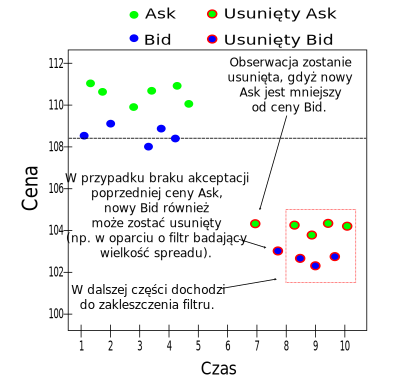
\includegraphics[width=0.6\textwidth]{wykresy/relacjaBIDASK.pdf}
%  \caption{Przypadek zakleszczenia się filtru spowodowany nagłym skokiem ceny.}
%  \label{fig:JUMP}
%\end{figure}

\subsection{Aktualizacja \MSpn}

Listing \ref{FiltrUpdate} przedstawia sposób aktualizacji średniego spreadu \MSpn:

\begin{algorithm}

\eIf{TickAccepted}
{ $\Delta t = t - lastTime$\\
\nlset{Uwaga 1}\label{uwg1ta}	$\phi = exp(\Delta t / \lambda)$\\
\nlset{Uwaga 2}\label{uwg2ta}	$\phi = max(\phi, \phi_{min})$\\
\nlset{Uwaga 3}\label{uwg3ta} 	$\phi = min(\phi, \phi_{max})$ \\ 
\nlset{Aktualizacja}\label{line:akt}	$\MSpn = \phi \cdot \MSpc + (1 - \phi) \Spt$
}
{
\nlset{Zabezpieczenie 3}\label{Zab3} \MSpn = \MSpc + RmVal\\
}


\caption{Algorytm aktualizacji \MSpn \label{FiltrUpdate}}
\end{algorithm}

Nowa wartość \MSpn jest ważoną średnią poprzedniej wartości i aktualnego spreadu. Przy czym  waga \Spt zależna jest od czasu pomiędzy dwiema ostatnimi obserwacjami (\ref{uwg1ta}). Im krótszy czas, tym wpływ nowej wartości spreadu jest większy. Dostosowywanie wartości $\phi$ odbywa się poprzez parametr $\lambda$ - większe wartości $\lambda$ oznaczają większy wpływ \Spt na wartość \MSpn. 

Dodatkowo wprowadzono parametr $\phi_{max}$, określający maksymalny udział aktualnego spreadu (\Spt) w \MSpn. Ma on na celu zapobieganie sytuacją zbytniego zmniejszenia się średniego spreadu gdy po dłuższym okresie jako pierwsze pojawi się tick którego spread względem starej przeciwnej ceny będzie bardzo mały, a spread dla następnych tików się powiększy, przez co kolejne obserwacje będą odrzucane, aż do momentu, odpowiedniego rozszerzenia się spreadu związnym z zabezpieczeniem \ref{Zab3}. W takiej sytuacji udział \Spt zostanie ograniczony do wartości $\phi_{max}$ Przykładowa sytuacja pokazana jest na rys. \ref{fig:deltaTime}. Jednocześnie należy zauważyć, że w pewnych przypadkach może to prowadzić do sytuacji w której spread będzie znacząco zawyżony. 

W tym przypadku ujawia się również dodatkowa słabość filtru mająca szczególne znaczenie w przypadku małej płynności instrumentu (rzadko pojawiających się danych). Dla pierwszej obserwacji po długim okresie spread może być liczony względem ceny która jest już nieaktualna, jednak nowa cena jeszcze się nie pojawiła \ref{fig:calcSpread}. W obecnym podejściu do fitracji danych, w którym założone jest działanie online (po sprawdzeniu tiku nie ma już do niego powrotu), obejście tego problemu jest bardzo trudne (o ile w ogóle możliwe). W pewnym stopniu rozwiązaniem jest wprowadzone wcześniej zabezpieczenie \ref{Zab1}, które nie dopuści do zakleszczenia się filtra, kosztem odrzucenia pierwszej obserwacji pojawiającej się po dłuższym okresie czasu (np. na otwarcie sesji).

Parametr $\phi_{min}$ określa minimalny udział \Spt w \MSpn. Przyspiesza on dostosowywanie się wartości średniego spreadu dla płynnego rynku. 

Linijka \ref{Zab3} jest kolejnym zabezpieczeniem przeciwko zakleszczeniu się filtru. Rozszerzenie spreadu o wartość $RmVal$ pozwala na samo-naprawienie się filtru w sytuacji w której nastąpił gwałtowny skok spreadu, kosztem kilku pierwszych obserwacji (por. \ref{fig:SpreadJump}). Takie zabezpieczenie posiada oczywistą wadę w przypadku całej serii złych danych - powolne rozszerzanie się średniego spreadu w końcu spowoduje, że obserwacje odstające zostaną uznane za poprawne (por \ref{fig:outSeries}). W tym przypadku należy dokonać wyboru dotyczącego wrażliwości filtru na długie serie złych danych, a szybkością samonaprawy w przypadku zakleszczenia. 


\end{document}